\documentclass[a4paper,14pt]{extarticle}
\usepackage{../../tex-shared/report-layout}

\renewcommand{\mylabnumber}{6}
\renewcommand{\mylabtitle}{Исследование алгоритмов сортировки данных методами
пузырька и Шелла, используемых при проектировании параллельных вычислительных
программных систем}
\renewcommand{\mysubject}{Теория распределенных систем и параллельных вычислений}
\renewcommand{\mylecturer}{Дрозин А.Ю.}

\begin{document}
\begin{titlepage}
    
    \thispagestyle{empty}
    
    \begin{center}
        
        Министерство науки и Высшего образования Российской Федерации \\
        Севастопольский государственный университет \\
        Кафедра ИС
        
        \vfill

        Отчет \\
        по лабораторной работе №\mylabnumber \\
        \enquote{\mylabtitle} \\
        по дисциплине \\
        \enquote{\MakeTextUppercase{\mysubject}}

    \end{center}

    \vspace{1cm}

    \noindent\hspace{7.5cm} Выполнил студент группы ИС/б-17-2-о \\
    \null\hspace{7.5cm} Горбенко К. Н. \\
    \null\hspace{7.5cm} Проверил \\
    \null\hspace{7.5cm} \mylecturer

    \vfill

    \begin{center}
        Севастополь \\
        \the\year{}
    \end{center}

\end{titlepage}

\section{Цель работы}
Программно реализовать и исследовать эффективность алгоритмов параллельной
сортировки с использованием функций библиотеки MPI в сравнении с
последовательными версиями тех же алгоритмов.

\section{Постановка задачи}
Выполнить разработку и отладку программы параллельной сортировки данных с
использованием вызовов требуемых функций библиотеки MPI в соответствии с
вариантом, указанным преподавателем. Дополнительно реализовать последовательный
вариант того же метода сортировки. Получить результаты работы программы в виде
протоколов сообщений, комментирующих параллельное выполнение процессов и их
взаимодействие в ходе выполнения. Оценить эффективность параллельного процесса
сортировки в сравнении с последовательным на том же наборе исходных данных.
Вариант №1 -- Четная-нечетная.

\section{Ход работы}
Текст программы:
\begin{lstlisting}
#include <iostream>

using namespace std;

void OddEvenSort(int* vector, int size);
void ShowVector(int vector[], int size);

int main()
{
    const int size = 15;
    int A[size] = { 41, 67, 34, 0, 69, 24, 78, 58, 62, 64, 5, 45, 81, 27, 61 };

    ShowVector(A, size);
    OddEvenSort(A, size);
    ShowVector(A, size);
}

void OddEvenSort(int* vector, int size)
{
    for (int i = 0; i < size; i++) 
    {
        if (i % 2 == 0) 
        {
            for (int j = 0; j < size; j += 2) 
            {
                if (j < size - 1) 
                {
                    if (vector[j] > vector[j + 1])
                    {
                        int tmp = vector[j];
                        vector[j] = vector[j + 1];
                        vector[j + 1] = tmp;
                    }
                }
            }
        }
        else 
        {
            for (int j = 1; j < size; j += 2) 
            {
                if (j < size - 1) 
                {
                    if (vector[j] > vector[j + 1])
                    {
                        int tmp = vector[j];
                        vector[j] = vector[j + 1];
                        vector[j + 1] = tmp;
                    }
                }
            }
        }
    }
}

void ShowVector(int vector[], int size)
{
    for (int i = 0; i < size; i++)
    {
        cout << vector[i] << " ";
    }
    cout << endl;
}

Программа 2. Параллельный метод сортировки:
#include <iostream>
#include <mpi.h>

using namespace std;

const int data_tag = 2001;
const int N = 15;

void ShowVector(int vector[], int size);
int* GetHalfVector(int vector[], int size, bool mode);
int Partition(int vector[], int start, int end);
void Quicksort(int vector[], int start, int end);
int* MergeSort(int firstVector[], int secondVector[], int firstVectorSize, int secondVectorSize);

int main(int argc, char** argv)
{
    // 41 67 34 0 69 24 78 58 62 64 5 45 81 27 61
    int rank, processes;
    MPI_Init(&argc, &argv);
    MPI_Comm_rank(MPI_COMM_WORLD, &rank);
    MPI_Comm_size(MPI_COMM_WORLD, &processes);
    MPI_Status status;

    int masterProcess = 0;
    int vector[N];
    int* sortedVector = new int[N];
    int blockSize = N / processes;
    int* blockVector = new int[blockSize];

    if (rank == masterProcess) 
    {
        for (int i = 0; i < N; i++)
        {
            vector[i] = 0 + rand() % 100;
        }

        cout << "Unsorted vector: ";
        ShowVector(vector, N);
        cout << endl;
    }

    MPI_Scatter(vector, blockSize, MPI_INT, blockVector, blockSize, MPI_INT, masterProcess, MPI_COMM_WORLD);

#pragma region DEBUG
    cout << "P" << rank << "-unsorted: ";
    ShowVector(blockVector, blockSize);
    MPI_Barrier(MPI_COMM_WORLD);
#pragma endregion

    Quicksort(blockVector, 0, blockSize - 1);

#pragma region DEBUG
    cout << "P" << rank << "-sorted: ";
    ShowVector(blockVector, blockSize);
#pragma endregion

    MPI_Barrier(MPI_COMM_WORLD);

    for (int i = 0; i < processes - 1; i++) 
    {
        if (i % 2 == 0) 
        {
            if (rank % 2 == 0) 
            {
                if (rank != processes - 1) 
                {
                    int* blockVectorFromNext = new int[blockSize];
                    MPI_Send(blockVector, blockSize, MPI_INT, rank + 1, data_tag, MPI_COMM_WORLD);
                    MPI_Recv(blockVectorFromNext, blockSize, MPI_INT, rank + 1, data_tag, MPI_COMM_WORLD, &status);

                    int* merged = MergeSort(blockVector, blockVectorFromNext, blockSize, blockSize);
                    blockVector = GetHalfVector(merged, blockSize * 2, 0);

#pragma region DEBUG
                    cout << "P" << rank << "-merged-sorted: ";
                    ShowVector(merged, blockSize * 2);

                    cout << "P" << rank << "-half: ";
                    ShowVector(blockVector, blockSize);
#pragma endregion

                    delete[] blockVectorFromNext;
                    delete[] merged;
                }
            }
            else 
            {
                int* blockVectorFromPrev = new int[blockSize];
                MPI_Send(blockVector, blockSize, MPI_INT, rank - 1, data_tag, MPI_COMM_WORLD);
                MPI_Recv(blockVectorFromPrev, blockSize, MPI_INT, rank - 1, data_tag, MPI_COMM_WORLD, &status);

                int* merged = MergeSort(blockVector, blockVectorFromPrev, blockSize, blockSize);
                blockVector = GetHalfVector(merged, blockSize * 2, 1);

#pragma region DEBUG
                cout << "P" << rank << "-merged-sorted: ";
                ShowVector(merged, blockSize * 2);

                cout << "P" << rank << "-half: ";
                ShowVector(blockVector, blockSize);
#pragma endregion

                delete[] blockVectorFromPrev;
                delete[] merged;
            }
        }
        else 
        {
            if (rank % 2 == 0) 
            {
                if (rank != 0) 
                {
                    int* blockVectorFromPrev = new int[blockSize];
                    MPI_Send(blockVector, blockSize, MPI_INT, rank - 1, data_tag, MPI_COMM_WORLD);
                    MPI_Recv(blockVectorFromPrev, blockSize, MPI_INT, rank - 1, data_tag, MPI_COMM_WORLD, &status);

                    int* merged = MergeSort(blockVector, blockVectorFromPrev, blockSize, blockSize);
                    blockVector = GetHalfVector(merged, blockSize * 2, 1);

#pragma region DEBUG
                    cout << "P" << rank << "-merged-sorted: ";
                    ShowVector(merged, blockSize * 2);

                    cout << "P" << rank << "-half: ";
                    ShowVector(blockVector, blockSize);
#pragma endregion

                    delete[] blockVectorFromPrev;
                    delete[] merged;
                }
            }
            else 
            {
                int* blockVectorFromNext = new int[blockSize];
                MPI_Send(blockVector, blockSize, MPI_INT, rank + 1, data_tag, MPI_COMM_WORLD);
                MPI_Recv(blockVectorFromNext, blockSize, MPI_INT, rank + 1, data_tag, MPI_COMM_WORLD, &status);

                int* merged = MergeSort(blockVector, blockVectorFromNext, blockSize, blockSize);
                blockVector = GetHalfVector(merged, blockSize * 2, 0);

#pragma region DEBUG
                cout << "P" << rank << "-merged-sorted: ";
                ShowVector(merged, blockSize * 2);

                cout << "P" << rank << "-half: ";
                ShowVector(blockVector, blockSize);
#pragma endregion

                delete[] blockVectorFromNext;
                delete[] merged;
            }
        }

        MPI_Barrier(MPI_COMM_WORLD);
    }

    MPI_Barrier(MPI_COMM_WORLD);
    MPI_Gather(blockVector, blockSize, MPI_INT, sortedVector, blockSize, MPI_INT, masterProcess, MPI_COMM_WORLD);
    MPI_Barrier(MPI_COMM_WORLD);

    if (rank == masterProcess) 
    {
        cout << endl << "Sorted vector: ";
        ShowVector(sortedVector, N);
    }

    delete[] blockVector;

    MPI_Finalize();

    return 0;

}

void ShowVector(int vector[], int size)
{
    for (int i = 0; i < size; i++)
    {
        cout << vector[i] << " ";
    }
    cout << endl;
}

int* GetHalfVector(int vector[], int size, bool mode)
{
    int* result = new int[size / 2];

    if (mode) 
    {
        copy(vector + size / 2, vector + size, result);
    }
    else 
    {
        copy(vector, vector + size / 2, result);
    }

    return result;
}

int Partition(int vector[], int start, int end)
{
    int pivot = vector[end];
    int pIndex = start;

    for (int i = start; i < end; ++i)
    {
        if (vector[i] < pivot)
        {
            swap(vector[i], vector[pIndex]);
            pIndex++;
        }
    }

    swap(vector[pIndex], vector[end]);

    return pIndex;
}

void Quicksort(int vector[], int start, int end)
{
    int* stack = (int*)malloc((end - start + 1) * sizeof(int));
    int top = -1;
    stack[++top] = start;
    stack[++top] = end;

    while (top >= 0)
    {
        end = stack[top--];
        start = stack[top--];

        int pivot_index = Partition(vector, start, end);

        if (pivot_index - 1 > start)
        {
            stack[++top] = start;
            stack[++top] = pivot_index - 1;
        }
        if (pivot_index + 1 < end)
        {
            stack[++top] = pivot_index + 1;
            stack[++top] = end;
        }
    }
}

int* MergeSort(int firstVector[], int secondVector[], int firstVectorSize, int secondVectorSize)
{
    int i = 0;
    int j = 0;
    int index = 0;
    int* result = new int[firstVectorSize + secondVectorSize];

    while (i < firstVectorSize && j < secondVectorSize) 
    {
        if (firstVector[i] < secondVector[j]) 
        {
            result[index] = firstVector[i];
            i++;
        }
        else 
        {
            result[index] = secondVector[j];
            j++;
        }
        index++;
    }

    while (i < firstVectorSize) 
    {
        result[index] = firstVector[i];
        index++;
        i++;
    }

    while (j < secondVectorSize) 
    {
        result[index] = secondVector[j];
        index++;
        j++;
    }

    return result;
}
\end{lstlisting}

Первым этапом был разработан последовательный алгоритм чет-нечетной сортировки.
Результат сортировки таким методом представлен на рисунке \ref{fig:result}.
\begin{figure}[H]
    \centering
    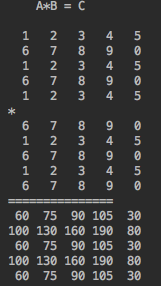
\includegraphics[width=.5\linewidth]{result}
    \caption{Результат выполнения последовательного алгоритма чет-нечетной сортировки}
    \label{fig:result}
\end{figure}

Далее было осуществлено моделирование параллельного алгоритма чет-нечетной
сортировки. Каждый этап был проведен вручную, что позволило полностью понять,
как работает данный алгоритм. Данные для сортировки были взяты из примера выше.
Результат показан на рисунке \ref{fig:modeling}.
\begin{figure}[H]
    \centering
    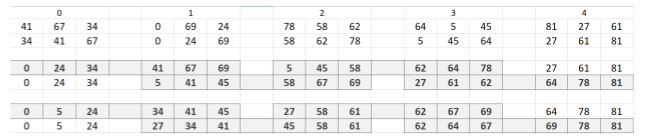
\includegraphics[width=\linewidth]{modeling}
    \caption{Результат моделирования параллельного алгоритма чет-нечетной сортировки}
    \label{fig:modeling}
\end{figure}

Как видим, из рисунка 2 следует, что существует processes – 1 итераций из четной
и нечетной фазы. На каждой четной фазе процессы (0 1), (2 3) и т.д. обмениваются
блоками и составляют общий массив и сортируют его, после этого каждый оставляет
себе половину по правилу: процесс с меньшим номером оставляет себе левую
половину, процесс с большим – правую. Таким же образом действуют процессы на
нечетной фазе, однако уже (1 2), (3 4) и т.д.

После всех итераций мы собираем данные с процессов и получаем отсортированный
массив.
\begin{figure}[H]
    \centering
    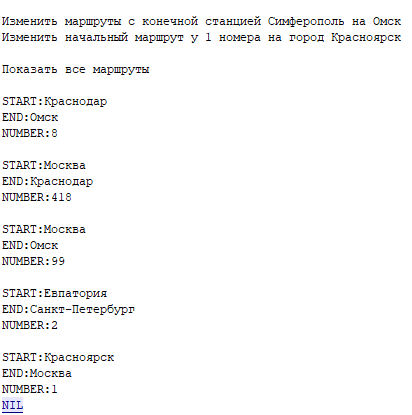
\includegraphics[width=.65\linewidth]{result2}
    \caption{Результат выполнения параллельного алгоритма чет-нечетной сортировки}
    \label{fig:result2}
\end{figure}

\section*{Выводы}
В ходе данной лабораторной работы были изучены основные понятия составления
параллельных методов сортировок их последовательных аналогов. Программно
реализован и исследован алгоритм чет-нечетной параллельной сортировки с
использованием функций библиотеки MPI в сравнении с последовательными версиями
тех же алгоритмов.
\end{document}